%
\section{System Operation}
\label{sect:operation}
%
\begin{figure}[htb!]
\begin{center}
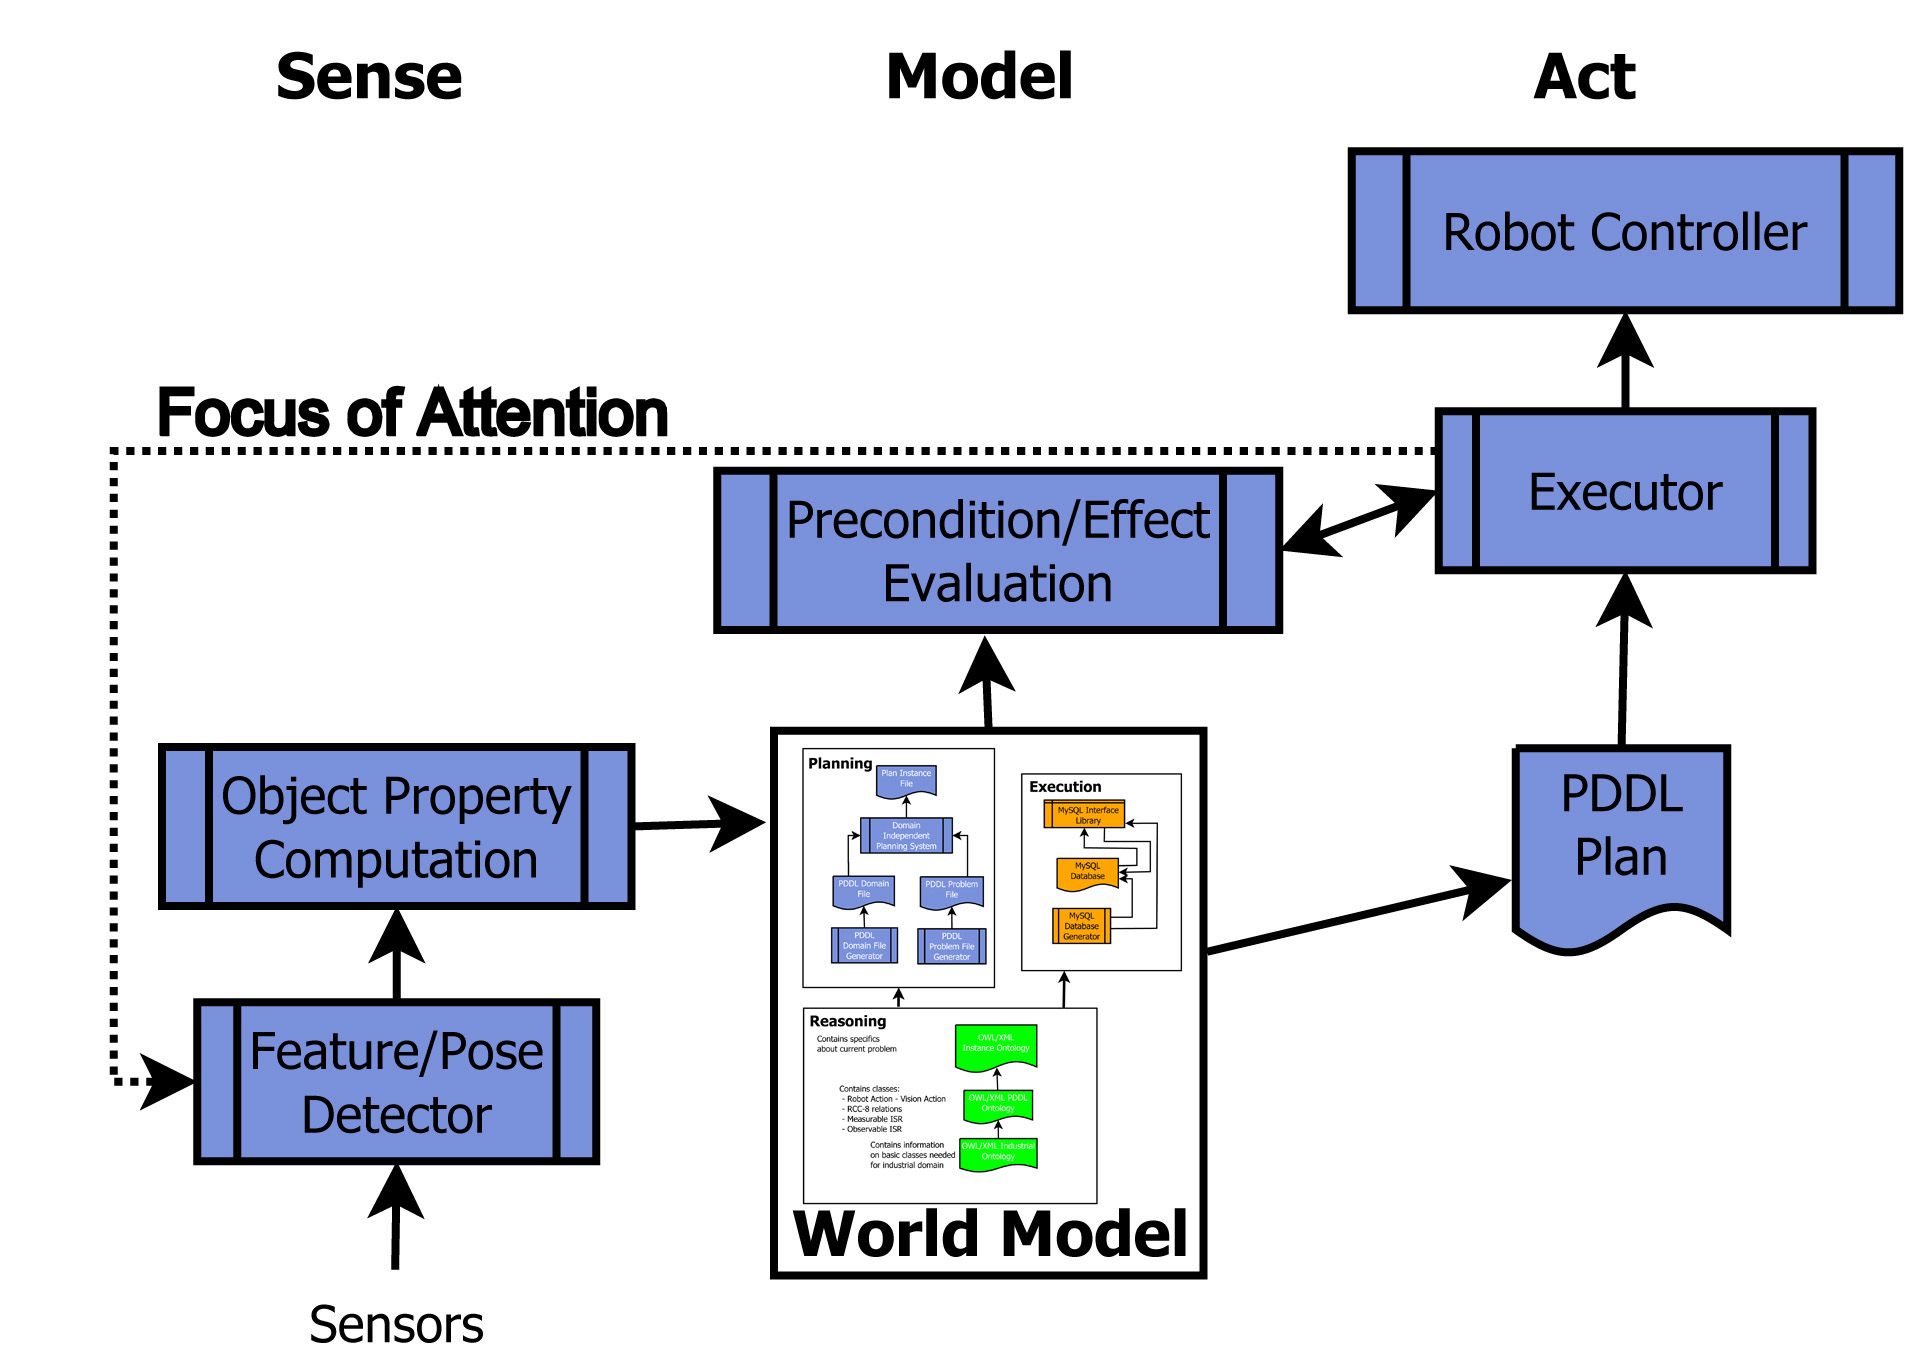
\includegraphics[width=8.5cm]{images/SenseModelAct.jpg}
\caption{Major components that make up the Sense--Model--Act paradigm of the kitting station.}
\label{fig:SenseModelAct}
\end{center}
\end{figure}
The kitting framework that has been implemented as part of this work 
is a deliberative intelligent system based on a single 
level or echelon of the hierarchal 4D/RCS 
reference model architecture \cite{Albus2000} and is
tightly coupled with a domain independent planning system. As shown
in Figure \ref{fig:SenseModelAct}, 4D/RCS 
follows a sense-model-act paradigm. 
%
\begin{figure}[htb!]
\begin{center}
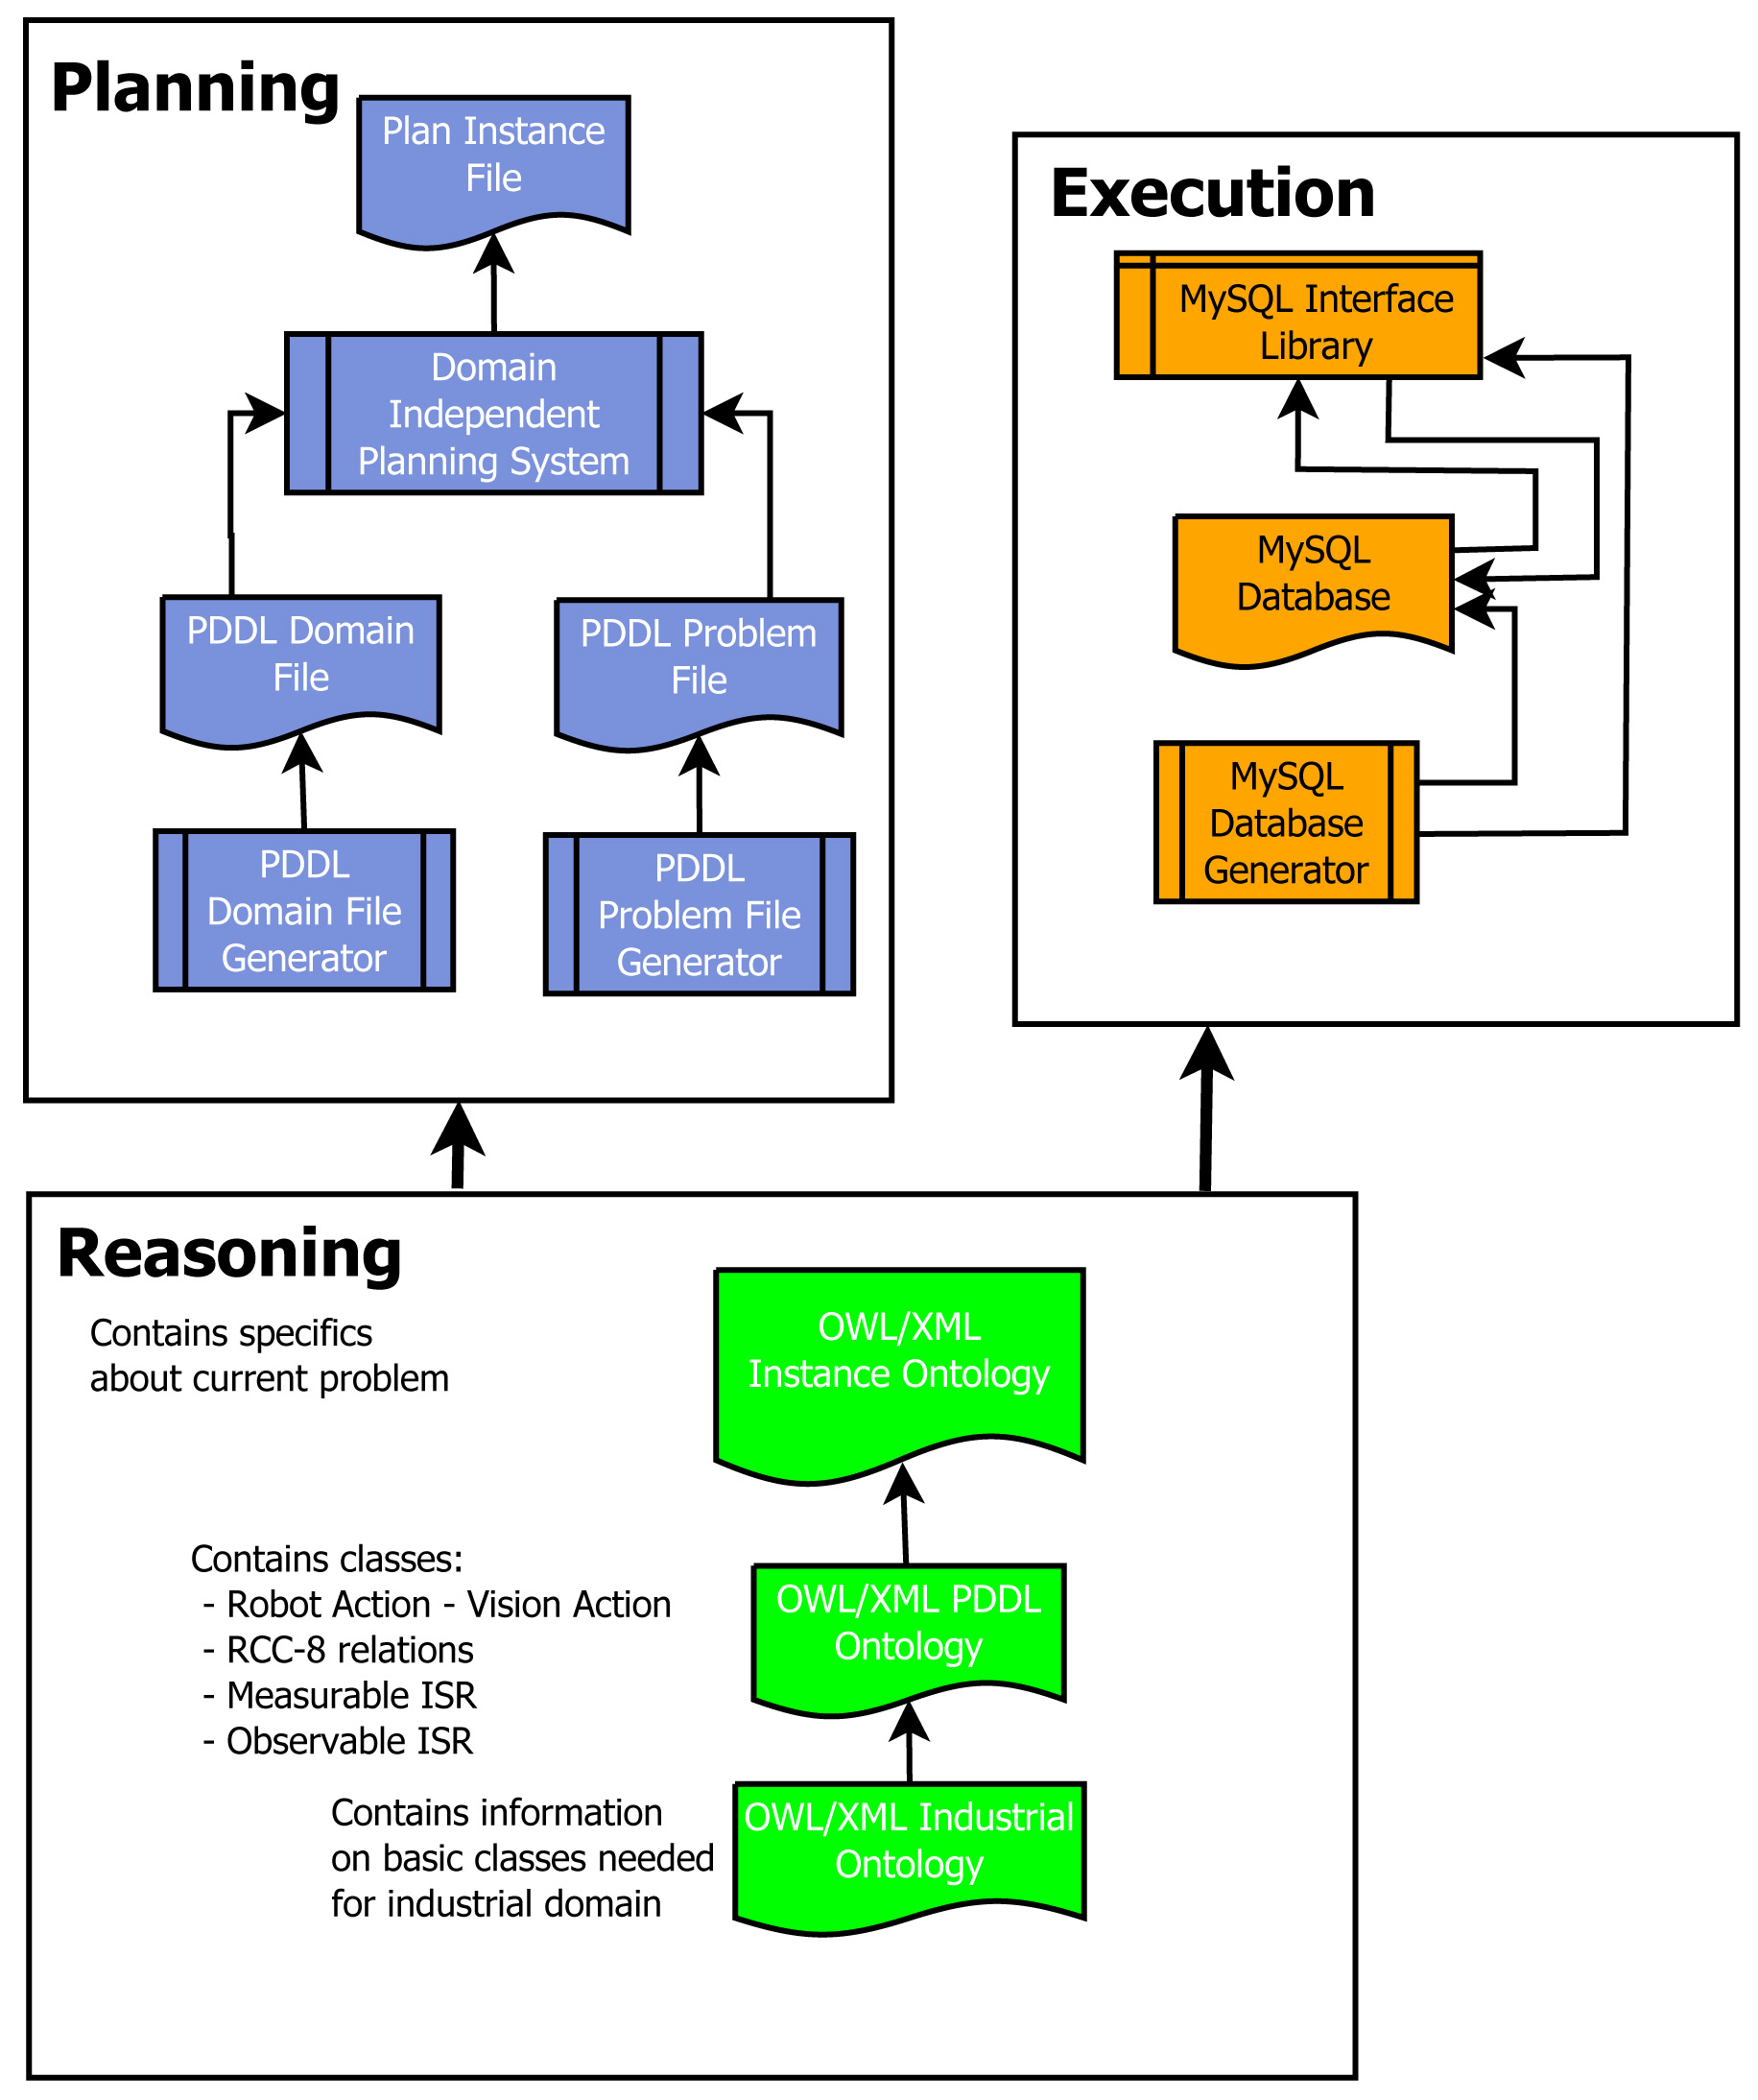
\includegraphics[width=12cm]{images/WorldModel.jpg}
\caption{System World Model - The world model contains a Reasoning section that is based on an ontology shown in green,
a Planning section that is based on a Planning Domain Definition Language (PDDL) specification shown in blue, and an Execution section that is based on a relational database (MySQL) shown in orange.}
\label{fig:WorldModel}
\end{center}
\end{figure}
%
A central feature of 4D/RCS is its world model. As shown in Figure \ref{fig:WorldModel},
the world model for this system may be decomposed into the three parts of
Reasoning, Planning, and Execution. All of the concepts necessary for the industrial
domain under test and for PDDL plan execution are encoded in the ontology that resides in the reasoning section of the model. The planning and execution sections of the model are automatically generated from this section.
%
\subsection{Reasoning}
The reasoning portion of the world model is designed to contain all of the information needed to reason over and solve complex industrial
problems. The knowledge is represented in an XML schema and is automatically translated into the Web Ontology Language (OWL) with
tools described in Kramer et al. \cite{kramer2014}. The  ontology is structured in three parts. The first part of the ontology contains generic information and classes that are needed for the domain of kit building. 
%
\begin{figure}[htb!]
\begin{center}
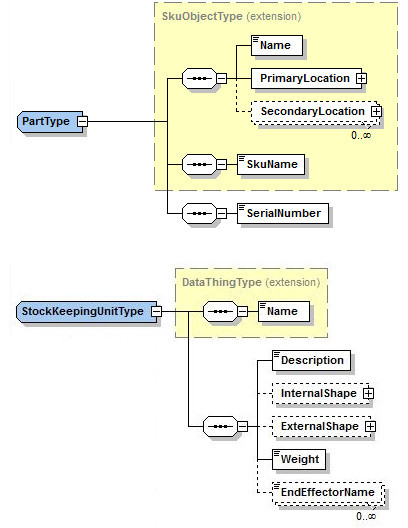
\includegraphics[width=8.5cm]{images/PartSKUV2.jpg}
\caption{Description of the PartType class that is designed to contain both static and dynamic information about particular parts and the StockKeepingUnitType class that contains static information about classes of parts.}
\label{fig:part}
\end{center}
\end{figure}
%
This area of the ontology contains information on basic elements such as a ``point" which is defined as a class that contains a name 
and a three-dimensional quantity, as well as complex types such as a ``part'', which is
shown in Figure \ref{fig:part}, and
contains elements such as the part's location and a name that references a stock keeping unit. The stock keeping unit contains static information on classes of parts such as the part's shape, weight, and the end effector that should be used for grasping the part. This information is utilized to create parameters for the Planning World
Model and the skeleton tables for the MySQL database of the Execution World Model.

Both static and dynamic information is represented in this
ontology and is automatically transitioned into the Planning and Execution areas of the world model. During system
operation,  dynamic information is updated in the Execution World Model.
More information on this portion of the ontology may be found in \cite{Balakirsky2012-1}.
%
\begin{figure}[htb!]
\begin{center}
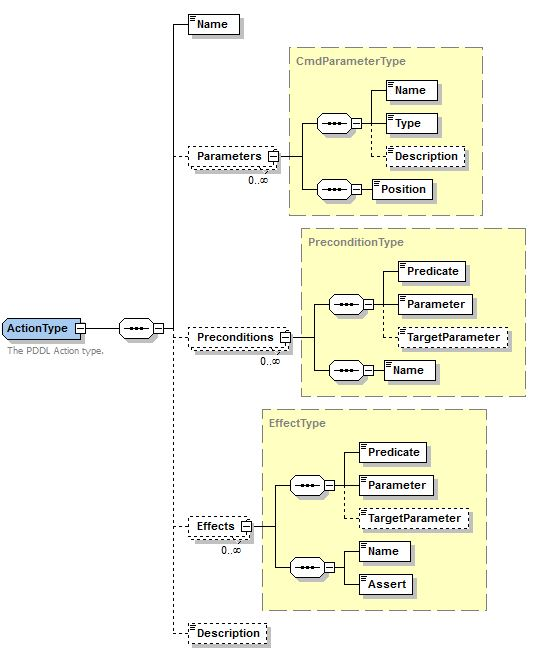
\includegraphics[width=8.5cm]{images/ActionType.jpg}
\caption{XML schema representation of a PDDL action. Contains
representations of the action's parameters, preconditions, and effects.}
\label{fig:ActionType}
\end{center}
\end{figure}
%

The second part of the ontology (known as PDDL ontology) contains the high-level concept of an action and all of the concepts 
that are required to support an action. Figure \ref{fig:ActionType}
depicts the template for the action representation. In addition,
this portion of the ontology contains information on the set of
functions that are hard-coded onto the robot and vision systems, and
templates for how these functions may be composed into higher-level
activities. More information on this action composition may be found
in Section \ref{sect:knowledge}. 

The third part of the ontology contains specific instances needed for a particular domain. All of the necessary information for the automatic generation of the PDDL domain file required by the planning system is contained in the combination of this instance ontology and the PDDL ontology. 

One of the goals of this framework is to introduce additional agility into industrial processes. Therefore,
partial information is accepted and even encouraged for this area of the ontology. For the example of a part shown in Figure \ref{fig:part}, information on the SKU, grasp points 
(part of the ExternalShape or InternalShape), and name would be expected to be available at runtime. Information on the location of the part (PrimaryLocation) may not
become valid until after a \textit{VisionCommand} has been executed
that has identified and located the particular part.
%
\subsection{Planning Model}
PDDL planners require a PDDL file-set that consists of two files that specify the domain and the problem.
From these files, the planning system creates an additional static plan file. Both the domain and problem file are able to be auto-generated from the reasoning section of the world model.

The generated static plan file contains a sequence of actions that will transition the system from the initial state to the goal state. In order to maintain flexibility, it is desired that detailed information that is subject to change should be ``late-bound'' to the plan. In other words, specific information is acquired directly before that information needs to be used by the system. This allows for last minute changes in this information. For example, the location of a kit tray on a work table may be different from run to run. However, one would like to be able to use the same planning sequence for constructing the kit independent of the tray's exact position.

To compensate for this lack of exact knowledge, the plans that are generated by the PDDL planning system contain only high-level actions. A representation of this plan may be stored in the ontology for future use.
% 
\subsection{Execution Model}
The execution world model is also built automatically from the
ontology. This world model consists of a MySQL database and C++ 
interfaces
that provide for easy access to the data. The table skeletons are 
generated from
the industrial ontology, and the tables are initially populated with 
information
from the instance ontology. During plan execution, the Executor 
guides the
sensor processing system in updating the information in this section 
of the world
model. All of the data structures encoded in the ontology are 
included in this
representation.
%
\subsection{Executor}
The overall framework
is coordinated by a module known as the executor
which receives its input from the 
domain independent planning system. 
Any one of a number of freely available
open source PDDL planners
such as the forward-chaining partial-order planning system from 
Coles et al. \cite{Coles.ICAPS.2010}
may be used in conjunction with this 
work. The planner may compute plans {\it a priori} that are
stored in a plan library for future retrieval, or may compute
new plans as conditions change that invalidate the currently
executing plan. The output of the PDDL planner is shown as
the driving input to the executor in the lower right-side of
Figure \ref{fig:SenseModelAct}.

%
\begin{algorithm}[h!]

 \KwData{ $kitToBuild$ }
 \KwResult{reports success or failure}
 	retrieve instance $PDDLInstance$ to construct kit $kitToBuild$\;
 	\For{each action $\textbf{A}$ in $PDDLInstance$}{
 		\For{each precondition $\textbf{P}$ of action $\textbf{A}$} {
			\If{$PredicateEvaluation(P)=false$}{
				report failure\;
			}
 		}
 		ExecuteAction($action \textbf{A}$)\; 
 		\For{each effect $\textbf{E}$ of action $\textbf{A}$} {
			\If{$PredicateEvaluation(E)==false$}{
				report failure\;
			}
 		}
 		report action success\;
 	}
 	report plan success\;
\caption{{\sc BuildKit} -- Sequences the actions necessary to build a kit.}
\label{fig:buildkit}
\end{algorithm}
%


In order to construct a kit, the executor steps through each
action in
the precomputed PDDL plan. The overall process, known as {\sc BuildKit} is described in Figure
\ref{fig:buildkit}. 

This process begins by retrieving a planning instance that has been 
precomputed to solve the construction of the requested kit (Line 1 of 
Figure \ref{fig:buildkit}). This PDDL
plan is an ordered sequence of actions with each action
containing types from the ontology as parameters. These
types represent generic classes and are not yet grounded
in specific instances that exist in the world. The PDDL
actions may be broadly categorized into actions that are
designed to ground objects to specific instances (Vision Actions)
and actions that are designed to manipulate grounded objects (Robot 
Actions). 

%
\begin{figure}[htb!]
\fbox{
\begin{minipage}{0.5\textwidth}
\begin{center}
Vision Actions
\end{center}
\begin{itemize}
\item look-for-endEffector-holder
\item look-for-endEffector
\item look-for-kitTray-holder
\item look-for-kitTray
\item look-for-workTable
\item look-for-part
\item look-for-slot
\end{itemize}
\end{minipage}
%
\begin{minipage}{0.5\textwidth}
\begin{center}
Robot Actions
\end{center}
\begin{itemize}
\item attach-endEffector
\item detach-endEffector
\item take-kitTray
\item place-kitTray
\item place-kitTray
\item take-part
\item place-part
\end{itemize}
\end{minipage}
}
\caption{Family of PDDL actions necessary to build a kit.}
\label{fig:PDDLActions}
\end{figure}

The set of these actions for the kitting domain may be seen in
Figure \ref{fig:PDDLActions}. For the domain of kitting,
the Robot Actions are used to
pick-up and place parts while the Vision Actions are used to
located the parts and part destinations. The
{\it for} loop beginning at Line 2 of Figure \ref{fig:buildkit} steps
through the execution of each of the actions from the PDDL plan. 
Before the action is
executed, predicates in the form of
preconditions are examined to assure that the action 
to be attempted
is valid. If any of the action's preconditions are not able to 
be validated,
a failure is reported; otherwise, the action is approved for execution.
Once the action has been executed, additional predicates in the form
of effects are examined to determine the success of the action.
If any of the action's effects are not able to be validated, a 
failure is reported. If the action was successful, the loop will
begin again with the next PDDL action. Once all of the actions have
been successfully executed, plan success will be reported (line 16 of
figure \ref{fig:buildkit}).

All of the steps of the {\sc BuildKit} algorithm can be hard-coded into a robotic
system as was reported in Balakirsky et al. \cite{Balakirsky2013}. This
creates a system that is flexible and agile in terms of the type of kit that
is being built, and the placement of parts, trays, and kits. However, if
a procedural change is required that necessitates a new action, the system
must be taken down and reprogrammed. For example, if a new "inspect-part"
operation was desired, this action would need to be programmed into the system's
vocabulary. The remainder of this article concentrates on techniques that
allow more of this information to be stored in the system's ontology and thus
allow even greater flexibility in what the system is able to accomplish without
changes in programming.
